% vim:syntax=tex

In this section we provide an overview of our methodology.
We first describe the changeset topic model on which we base our work.
We then describe the process by which we mine the data
needed to build instances of this model.

\subsection{Changeset Topic Modeling}
\label{sec:changesets}

\subsection{Source Code Document Extraction}
\label{sec:extract}

We use the following linguistic model.
A \textit{word}
is the basic unit of discrete data in a software lexicon and
is a sequence of letters.
A \textit{token} is a sequence of non-whitespace characters
containing one or more words.
An {\it entity} is a named source element such as a method,
and an \textit{identifier} is a token representing the name of an entity.
\textit{Comments} and \textit{literals} are sequences of tokens
delimited by language-specific markers (e.g., /* */ and quotes).
The \textit{document} which corresponds to a class is a sequence of words $d = (w_1, \ldots, w_m)$,
and a \textit{corpus} is a set of documents (i.e., classes) $D = (d_1, \ldots, d_n)$.


% TODO fix this to say LDA instead of Mallet
\begin{figure*}
\vspace{2mm}
\centerline{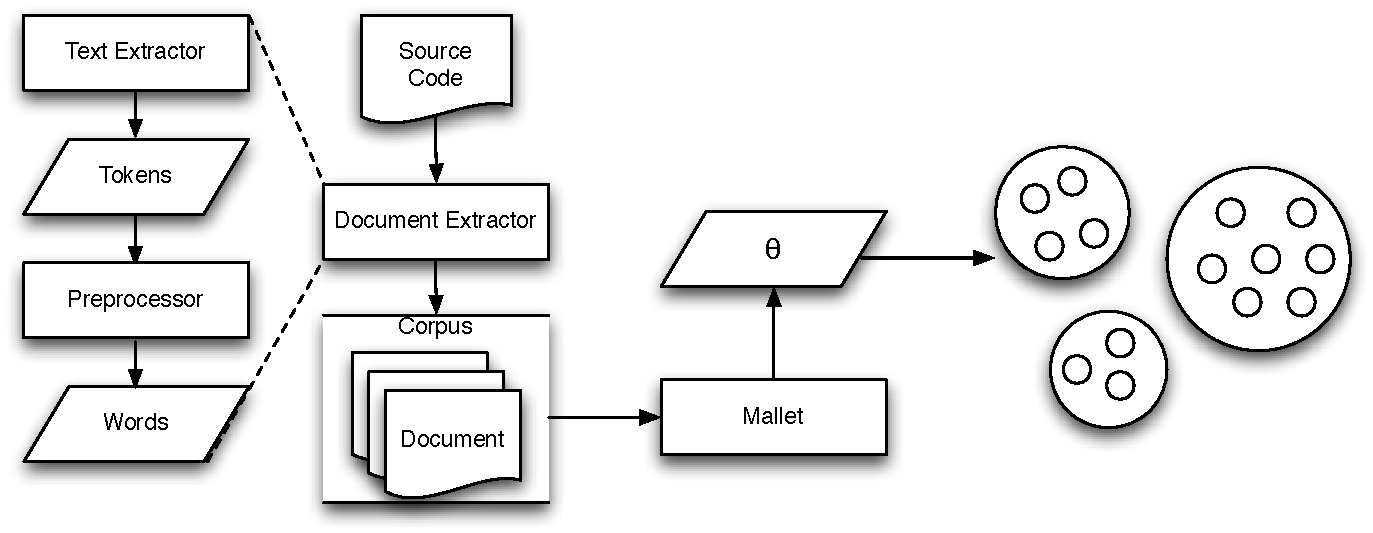
\includegraphics[width=.8625\textwidth]{Clustering}}
\caption{The source code document extraction and topic modeling processes.}
\label{fig:extract}
\vspace{-2mm}
\end{figure*}

The left side of Figure~\ref{fig:extract} illustrates the source code document extraction process.
A document extractor takes source code as input and produces a corpus as output.
Each document in the corpus contains the words associated with a class.
The text extractor is the first part of the document extractor.
It parses the source code and produces a token stream for each class.
With regard to Java, we consider an interface or enum name to be a class name.
The preprocessor is the second part of the document extractor.
It applies a series of transformations to each token and
produces one or more words from the token.
The transformations~\cite{Marcus-etal:04,Marcus-Menzies:10}: % that we use are:
\begin{itemize}
   \item {\it Splitting}: separate tokens into constituent words
         based on common coding style conventions (e.g., the use of camel case or underscores)
         and on the presence of non-letters (e.g., punctuation or digits)
   \item {\it Normalizing}: replace each upper case letter with the corresponding
         lower case letter
   \item {\it Filtering}: remove common words such as articles (e.g., `an' or `the'),
         programming language keywords, standard library entity names, or short words
\end{itemize}
We build a corpus from a single snapshot of a software system and for all
commits leading up to that snapshot.
In particular, for the study we present in this paper,
we use the commit or tag corresponding to the snapshot (release) of each subject system.

